
\chapter{Imaging Breast Cancer: Chest Wall Effects}
\label{Chap:3_chestwall}
\vspace{-5mm}
\section{Introduction}
\vspace{-5mm}
Although various forms of diffuse optical tomography (DOT) have been employed to derive spatial maps of physiological features in the human breast with some success, the fidelity of these images is compromised by boundary effects such as those that arise from data obtained near the subject's chest wall. 

The breast is sometimes approximated as a slab, which allows the formulation of imaging problem with analytical Green's functions. The chest wall falls within the vicinity of the breast through which light can travel. Furthermore, from a general diffuse optics viewpoint, the very existence of the chest wall breaks the natural symmetry of the slab geometry, a symmetry which is often utilized when formulating Green's functions for the imaging problem. The chest wall introduces perturbations into the inverse problem that become more important as the source and detector locations move away from the nipple region and closer to the chest.

The DOT community has not dealt systematically with the influence of the chest wall. Dealing with these chest wall issues is the primary purpose of the research described in this Chapter, which is based on and expands upon my publication in the Journal of Biomedical Optics \cite{Ban2013}.  The remainder of this sub-section provides a brief perspective about the whole of my work on this problem. Following the present section, it is organized as follows: in Section~\ref{sec:3_exp} the experimental set-up is described in detail;  Section~\ref{sec:3_methods} explains our approaches to data restriction; Section~\ref{sec:3_results} presents the results, and Section~\ref{sec:3_summary} contains a brief discussion about the findings and implications of the work.
\\ \indent
Specifically, as part of our effort to translate DOT into the clinic, I set about to explore the effect of the chest wall in a systematic study at the optical bench. I assessed image quality of two types of DOT reconstructions: fast data-intensive analytic inversions and algebraic linear DOT. The investigation employed tissue phantoms with sub-centimeter targets in the presence of large absorbing regions that mimic the chest wall. My experiments show that this chest wall phantom can introduce image artifacts, and that these artifacts are especially severe for features near the boundary region.  The responses are fully characterized, and I show how these artifacts can be mitigated by exclusion of data near the chest wall. As part of this effort, in addition to exploring the utility of well-understood analytic inversions, I introduce and demonstrate a linear algebraic reconstruction method that is well suited for very large data sets (i.e., large data sets characteristic of CCD-based imagers); I study the performance of this algorithm for the first time as a function of distance from the phantom chest wall.

Here we employ linear image reconstruction methods and take measurements using continuous-wave (CW) illumination. In principle, one could also resort to time-~\cite{Patterson1989,Benaron1993,Andersson-Engels1990,Jacques1989,Schmidt2000,Ntziachristos1998} or frequency-domain~\cite{Gratton1990,Fishkin1993,Chance1998,Pogue1994} measurements and nonlinear reconstruction methods~\cite{Arridge1999,Markel2003a} to obtain a reconstruction of the target and the chest wall phantom simultaneously; however, these approaches require more expensive and complex instrumentation, as well as more time-consuming computational schemes.

The algorithms and experimental apparatus employed for these studies were carefully chosen to provide “best case” scenarios for breast imaging. It has been demonstrated that image quality in DOT~\cite{Wang2005,Konecky2008a,Bonfert-Taylor2012}, and in other imaging modalities such as inverse diffraction~\cite{Chaillat2012}, can be significantly improved by utilization of large data sets for the reconstruction. Furthermore, it has been shown that the plane-parallel transmission geometry is particularly well suited for utilization of larger data sets. The plane-parallel transmission geometry benefits from the possibility of non-contact source scanning~\cite{Schulz2003,Ripoll2003,Ripoll2004,Turner2005,Wang2005} and detection where a collimated laser beam can be scanned on one side of the sample for illumination, and is paired with a CCD camera for parallel detection.

A characteristic feature of such non-contact scanning approaches is the availability of very large data sets with up to $\sim 10^9$ independent measurements, e.g., with $\sim 10^3$ source positions and $\sim 10^6$ CCD pixels per source. Unfortunately, utilization of data sets consisting of more than $\sim 10^5$ independent measurements presents a serious computational challenge for traditional inversion methods, primarily due to data storage requirements. For this reason, theorists in the DOT community are motivated to develop new (and fast) algorithms capable of reconstructing very large data sets, albeit in simple imaging geometries (including the slab geometry) \cite{Markel2001,Markel2002,Markel2003,Markel2003a,Markel2004}. Numerical simulations~\cite{Markel2002} have explored some aspects of these methodologies, and they also indicate that large image windows (i.e., wide-field illumination and detection) are required to achieve optimal resolution. For example, the simulations suggest that the dimensions on both sides of the slab, wherein sources are scanned and CCD-detectors collect data, ideally, should be larger by a factor of approximately $3$ in both transverse directions compared to the slab thickness.  In practice, experimental studies have shown that a somewhat smaller ratio can be used and the ultimate limits will be due to the presence of noise and other imperfections of the imaging system~\cite{Wang2005,Konecky2008a}. My experiments employ this type of ideal experimental geometry and data generation/collection scheme with the additional complication of the chest-wall phantom. Thus my research helps to set best-case bounds for DOT breast imaging.

The tissue phantoms used for the experiment are similar to many that have been utilized with success in the DOT community for preclinical, {\em in vitro} investigations that ascertain the strengths and limitations of various image reconstruction schemes~\cite{Culver2003,Pogue2006,Cerussi2012}. One advantage of the present tissue phantom experiment is that it is possible to compare reconstructions obtained under similar conditions but with different imaging windows and spatial sampling, some of which would be difficult to realize {\em in vivo}. Thus, based on this single set of experimental results, I am able to discuss and compare two (or more) approaches for image reconstruction of large data sets under conditions of large/small imaging windows. In this way, one can more fully explore methods to ameliorate chest wall effects.
\clearpage
\section{Experiment and Setup}
\label{sec:3_exp}
In this sub-section, I will describe details of the experimental set-up including illumination, detection, and mechanical features of the tissue phantom. The experimental apparatus is shown in  Fig.~\ref{fig:chestwallschem}.
\begin{figure}[h]
\centering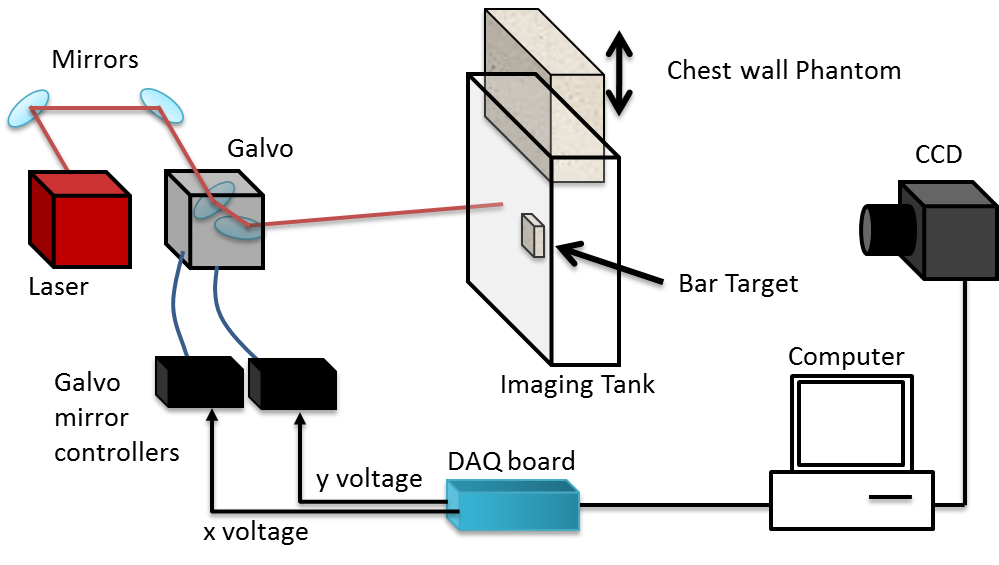
\includegraphics[width=14cm]{./figures/3_Chestwall/chestwallschem.png}
\caption[Schematic of the chest wall experiment]{Schematic of the experimental setup at the optical bench. A CW $785\,{\rm nm}$ laser source is raster scanned on one side of the imaging tank. The transmitted light on the detection plane is collected in parallel by a CCD and then binned (flexibly) for each source position.}
\label{fig:chestwallschem}
\end{figure}
\subsection{Light source}
Source illumination light is derived from a collimated $785$nm $90$mW  diode laser (Thorlabs, L785P090). The laser is coupled to a 2D galvonometer scanner (Thorlabs, GV012). The diode laser output is temperature sensitive, and therefore it is temperature controlled using a diode laser mount (Thorlabs, TCLDM9) and a temperature controller (ILX lightwave, LDT-5525) with custom cable for different pin configurations (required when using different brands for the mount and controller). The laser is current driven at $160\,{\rm mA}$ using the diode laser controller (Thorlabs, LDC500). The wavelength of the laser is $785\,{\rm nm}$. The output of the beam is collimated (Thorlabs, C140TMD-B) on the laser mount and is then focused, over a $2\,{\rm m}$ length, to a $0.5\,{\rm mm}$ spot size onto the source plane of the imaging tank.

The beam is raster scanned across this source plane of the imaging tank. Specifically, the collimated laser light is aligned with a pair of mirrors into the galvo scanner which raster scans a $35\times 35$ square grid with a $4\,{\rm mm}$ spacing covering an area of $13.6\times 13.6\,{\rm cm}^2$ on the inner side of the source window of the imaging tank. The galvo is controlled with a pair of drivers (one for each mirror). Voltages can be applied to the driver card to change the angle of the mirrors. Each mirror has a maximum angular displacement of $\pm 20^o$, and $1 \rm{V}$ moves the mirror $1^o$. Resistor pots on the driver were utilized to scale the voltage down (to $0.5 \rm{V}/1^o$) and to add an offset (as needed). A DAQ board (National Instruments, USB-6251) was used to output two distinct voltages (through its analog output channels a0 and a1) to the galvo scanner in series for each source position.

\begin{figure}[h]
\centering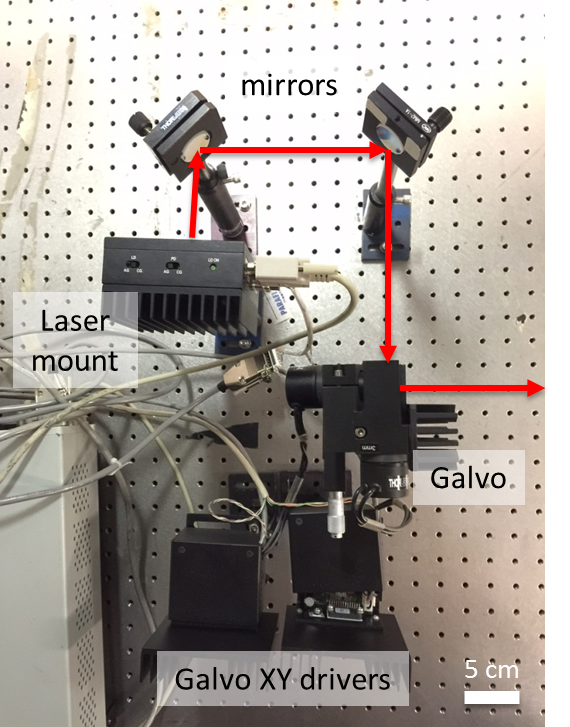
\includegraphics[width=7cm]{./figures/3_Chestwall/FSsource.png}
\caption[Photograph of the freespace laser and source position control setup]{Photograph of the laser and source position control setup. The diode laser is mounted on a TEC cooled mount with collimating lens that outputs the beam to a pair of mirrors which redirects the beam onto the galvo mirrors for scanning.}
\label{fig:FSsource}
\end{figure}

\subsection{Imaging Tank}
The imaging tank shown in Fig.~\ref{fig:chestwalltank} is designed specifically for the chest wall experiment. The tank is composed of aluminum walls on three surfaces (i.e., the bottom plate and two side plates) with acrylic windows in the input and output planes, and an opening at the top. The latter opening permits loading of Intralipid, targets and the chest wall phantom. In addition, a spigot is built into the side for easy draining and cleaning of the tank. The inner dimensions of the tank are $44\times 44\times 6\,{\rm cm}^3$. The $6\,{\rm cm}$ thickness of the tank was chosen to be close to the average compression used in our DOT clinical studies~\cite{Choe2009, Culver2003}. The unit has a removable black Delrin target holder which lines the walls of the tank, and it has evenly spaced holes that can be threaded with filamentous fishing lines to suspend various phantoms within the tank. These fishing lines hold bar targets (described in Section~\ref{sec:chestphant}). The windows are designed to be swappable and are lined with o-rings for water tight sealing. In this experiment a pair of $1/2-{\rm inch}$ acrylic windows were used. The top of the tank has optical posts that hold an aluminum plate which, in turn, holds a pair of threaded rods from which the chest wall phantom is suspended downwards.
\begin{figure}[h]
\centering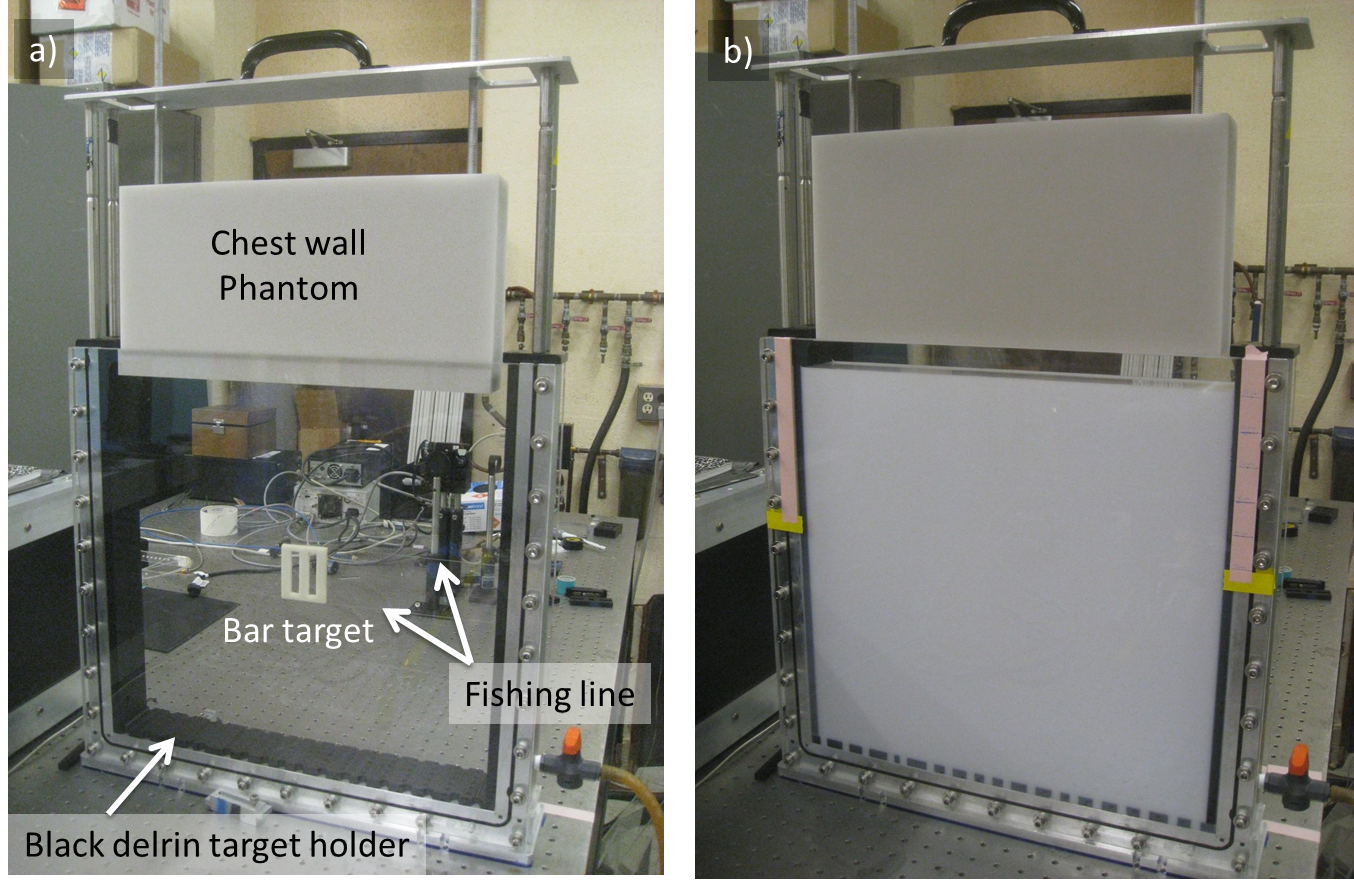
\includegraphics[width=14cm]{./figures/3_Chestwall/chestwalltank.png}
\caption[Photograph of the chest wall imaging tank]{Photograph of the imaging tank. a) The bar target is suspended below the chest wall phantom with fishing lines. b) The tank filled with Intralipid solution.}
\label{fig:chestwalltank}
\end{figure}

\subsection{CCD Detection}
For each illuminated source position, transmission data is collected on the opposite side of the tank over a $21.2\times 21.2\,{\rm cm}^2$ field-of-view (FOV) area. These data are collected with a CCD camera (Andor, DV887ECS-UV, lens $25\,{\rm mm}\ {\rm F}/0.95$). The FOV is effectively mapped to a grid of $512\times 512$ CCD pixels. This mapping yields a corresponding detected rectangular grid on the output surface of the tank with spacing $p=0.416\,{\rm mm}$. The CCD typically employed an exposure time of $500\,\rm{ms}$ at 16-bits (for a total of $2^{16}\sim64\rm{K}$ counts) with $1\times1$ binning. The total measurement time per scan was $\sim 11\,\rm{min}$.
\begin{figure}[h]
\centering
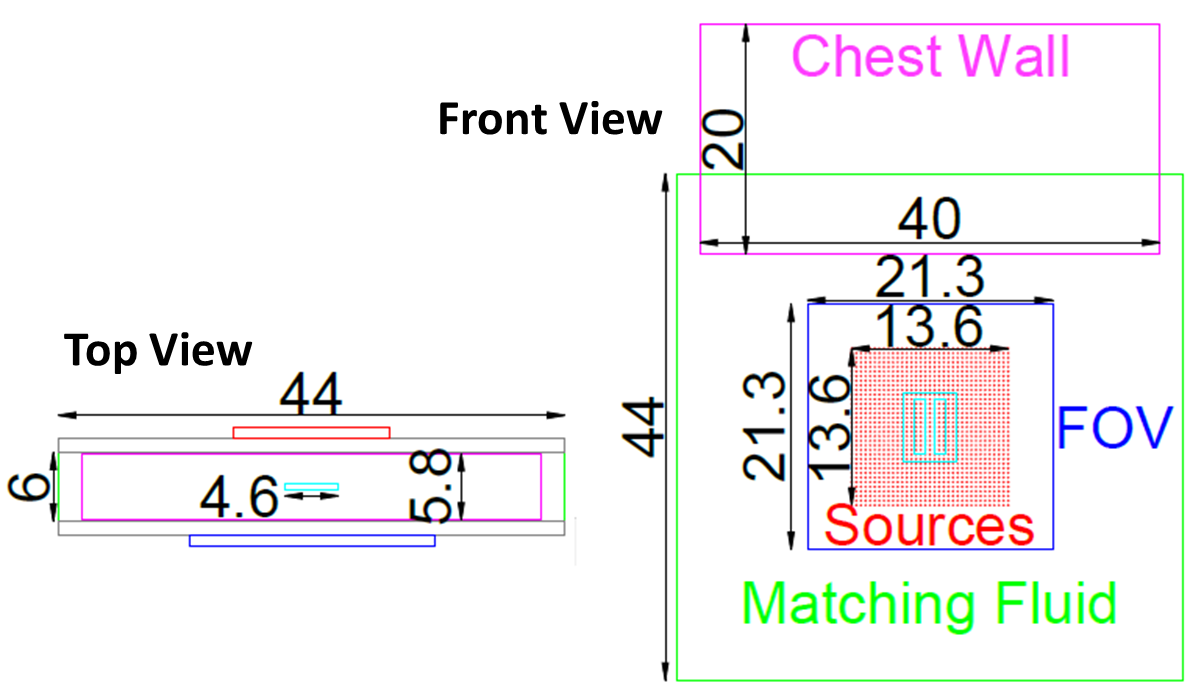
\includegraphics[width=11cm]{./figures/3_Chestwall/chestwalldim.png}
\caption[Schematic of the imaging tank with dimensions given in units of $\rm{cm}$]{Schematic of the imaging tank with dimensions given in units of $\rm{cm}$. The red sources make up a $13.6\times 13.6\,\rm{cm}$ grid within the blue $21.3\times 21.3\,\rm{cm}$ field of view of the CCD. The green dimensions are the tank size and the purple dimensions are those of the chest wall phantom.}
\label{fig:chestwalldim}
\end{figure}

\subsection{Phantoms: Bar Target and Chest Wall}
\label{sec:chestphant}
The bar target is made of silicon rubber (RTV-12, General Electric), titanium oxide (T-8141, Sigma-Aldrich) and carbon black (Raven 5000 Ultra Powder II). It has absorption coefficient $\mu_{\rm a}=0.2\,{\rm cm}^{-1}$ and reduced scattering coefficient $\mu_{\rm s}^\prime = 7.5\,{\rm cm}^{-1}$.  The tank is filled with an indian ink and intralipid solution ($\mu_{\rm a} = 0.05\,{\rm cm}^{-1}$ and $\mu_{\rm s}^\prime = 7.5\,{\rm cm}^{-1}$); these background optical properties are similar to those used in previous {\em in vitro} and clinical research. The contrast between the target and the surrounding fluid is purely absorptive with ratio of about 4. The bar target is suspended in the mid-plane of the tank ($3\,{\rm cm}$ from either surface) using the fishing line. 

A chest wall phantom (Biomimic, INO) with $\mu_{\rm a} = 0.1\,{\rm cm}^{-1}$ and $\mu_{\rm s}^\prime = 5.0\,{\rm cm}^{-1}$ and dimensions $40\times 20\times 5.8\,{\rm cm}^3$) is suspended at various distances, $d$, from the top edge of the bar target ($d=2$, $5$, $8$, $11$, $14$, $17\,{\rm cm}$) as shown in Fig.~\ref{fig:chestwallFOV} (a). The optical properties of the chest wall phantom were chosen to mimic muscle tissue~\cite{Ardeshirpour2010, Kienle1999,Taroni2003}. Thus both absorptive and scattering contrast exist between the chest wall phantom and the background fluid. The bar target and the chest wall phantom are shown in Fig.~\ref{fig:targets}.  Note that the chest wall phantom almost entirely fills the imaging tank; the clearance between the chest wall phantom and the inner surfaces of the tank is $1\,{\rm mm}$ on both sides.

\begin{figure}[t]
\centering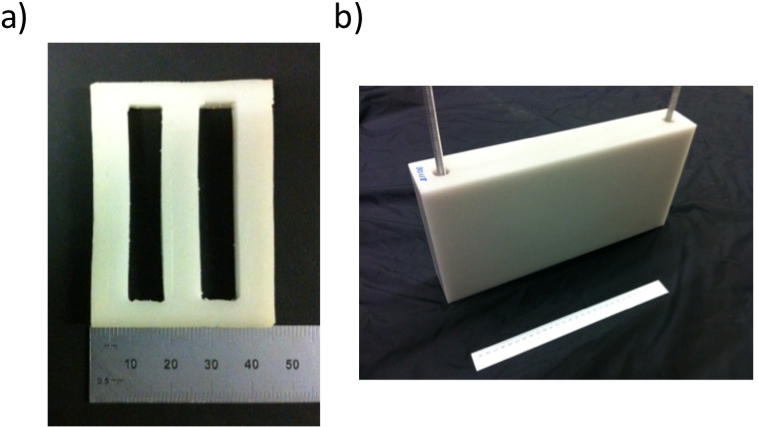
\includegraphics[width=10cm]{./figures/3_Chestwall/chestwallphant.pdf}
\caption[Phantoms used in chest wall experiment]{\label{fig:targets}
Phantoms used in the experiment. a) $6\,{\rm mm}$ thick bar target with $\mu_{\rm a}=0.2\,{\rm cm}^{-1}$ and $\mu_{\rm s}^{\prime}=7.5\,{\rm cm}^{-1}$ has slots $48\,{\rm mm}$ tall and $9\,{\rm mm}$ wide. The outer dimensions are $60\times 50\,{\rm mm}^2$. b) The chest wall phantom with $\mu_{\rm a}=0.1\,{\rm cm}^{-1}$ and $\mu_{\rm s}^{\prime}=5.0\,{\rm cm}^{-1}$.  }
\end{figure}

\section{Methods}
\label{sec:3_methods}
The experiments are straightforward. I first fill the tissue phantom tank with the background Intralipid suspension, and I collect baseline image data by cycling through each of the source positions and deriving a CCD-image output for each source position. Then I introduce the bar target into the suspension, and I insert the chest wall phantom into the suspension above the bar target (from the top). I then carry out another imaging measurement, i.e., obtaining CCD images while cycling through the source positions, with the bar target and chest wall phantom in the suspension and separated by a fixed distance. Lastly, I vary the distance between the bar target and the chest wall phantom and repeat the imaging procedure; I do this for multiple target-wall separation distances.

The data from the reference measurement and with the phantoms present are denoted by $I(\mbf{r}_d, \mbf{r}_s)$ and $I(\mbf{r}_d, \mbf{r}_s)$ (Eqns.~(\ref{eqn:Intensity1}) amd (\ref{eqn:Intensity2}) from Chapter 2) where $\mbf{r}_d$ $\mbf{r}_s$ which are the two dimensional vectors specifying the lateral positions of the detector and source on the respective surfaces of the tank. Image reconstruction is carried out using the methods described in Chapter 2 (see Section~\ref{sec:Analytic} and \ref{sec:Algebraic}). In this way, full 3D DOT reconstructions of the breast phantom and bar target are obtained as a function of the distance between the chest wall phantom and the bar target. This methodology permits characterization of the utility of the various methods in the presence of the chest wall, and it also permits exploration of selective data rejection schemes to ameliorate image artifacts. Below, I will describe this data rejection process in more detail.

In practice, a typical DOT measurement necessarily involves some rejection of data, i.e., rejection of data from source-detector pairs that are deemed unreliable or too noisy ~\cite{Blasi2007,Franceschini2007,Roche-Labarbe2010,Orihuela-Espina2010}. This data rejection could be a result of signals that are too small, uncontrolled fluctuations of the apparatus/subject, etc. In the usual approach, data are rejected based on {\em a priori} knowledge or a statistical model without specific regard for the location of the rejected source-detector pairs. In the present case, data restriction is used with a somewhat different goal to minimize systematic error effects due to the chest wall. Here particular data are rejected based solely on location. The purpose is not to suppress noise in the strictest sense, but rather to investigate the effects of imaging window restrictions and the effects of the proximity of the chest wall phantom and bar target on the quality of the image reconstructions. Importantly, the positions and distances of sources and detectors in close proximity to the chest wall are explored to determine which of them can be used, i.e., which source-detector pairs lead to reconstructions wherein the target is not significantly distorted or contaminated by chest wall systematics.

The distance between the top of the bar target and the bottom of the chest wall phantom as indicated in the figure is denoted $d$. Data is collected for $d=2$, $5$, $8$, $11$, $14$, and $17\,{\rm cm}$. The various data sets are graphically illustrated in Fig.~\ref{fig:chestwallFOV}. In Fig.~\ref{fig:chestwallFOV}(b), red lines show the positions of the lower edge of the chest wall phantom corresponding to different values of $d$ which fall within the CCD field-of-view (e.g, $d=8$, $5$, and $3\,{\rm cm}$). In this figure the source positions are shown as a small square grid of dots. Note, the image is to scale, and a slice of the sample reconstruction is superimposed with the drawing in order to indicate the target shape and position. The large dark blue square corresponds to the field-of-view (FOV) of the CCD camera. 
\begin{figure}[t]
\centering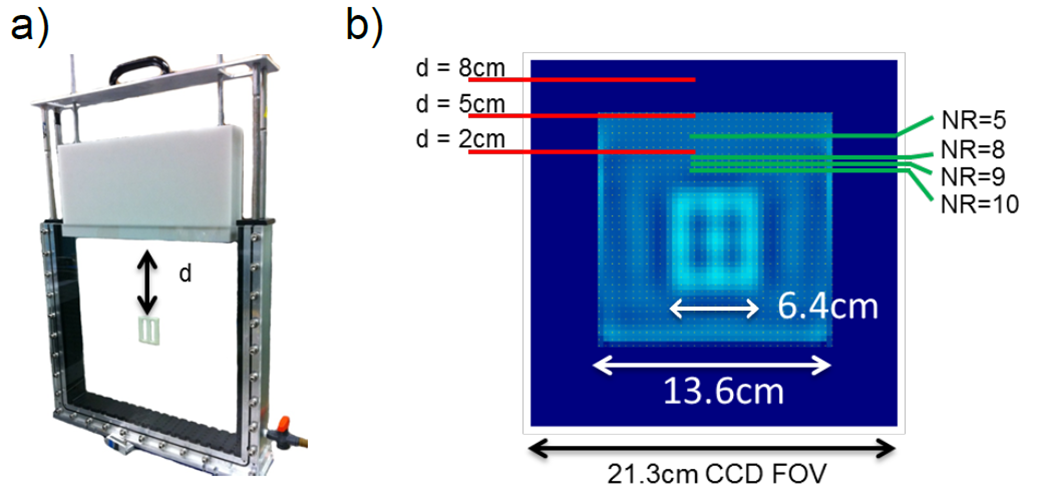
\includegraphics[width=13cm]{./figures/3_Chestwall/chestwallFOV.png}
\caption[Models for data restriction]{\label{fig:chestwallFOV}
Models for data restriction. (a) Photograph of the drained imaging tank illustrating the position the bar target with respect to the chest wall phantom. (b) Schematic of the imaging tank. (c) Illustration of the various data sets used for the reconstructions. The dark blue square is the CCD FOV; the inner light blue square indicates the reconstruction region. White dots in a square grid indicate the source positions. To illustrate the target shape and position, a slice of a sample reconstruction is superimposed with the drawing. Red lines indicate the three lowest positions of the chest wall phantom (other positions are outside of the CCD FOV), and the green lines illustrate the restricted data sets wherein all the sources and detectors situated above a given green line have been discarded.}
\end{figure}

The linear reconstruction techniques (analytical and algebraic) discussed in Section~\ref{sec:linearrecon} are applied to the experimental data obtained using the apparatus described above. These techniques are able to handle large data sets and permit comparison to previous work \cite{Konecky2008a}. The maximum number of independent source-detector pairs is $(512\times 35)^2\simeq 3.2\times 10^8$. However, only a fraction of this data (albeit still a large data set) was used in the reconstructions. Some data was eliminated by ``windowing'' (i.e., in the algebraic image reconstruction); other data were eliminated by a relatively sparse sampling of the detectors (e.g, in the algebraic reconstructions, every second detector was used), and still other data were eliminated by numerical data restrictions (described below). Thus the maximum data set utilized for reconstruction (in this case, for the algebraic reconstruction) was still very large, i.e., it consisted of $\simeq 2\times 10^7$ measurements.

In obtaining algebraic reconstructions, the reconstructed volume was divided into cubic voxels. The voxel size $h$ was taken to be equal to 8 CCD pixels $p$. Thus, $h=8\times 0.416\,{\rm mm}\simeq 3.3\,{\rm mm}$. The grid consisted of $41\times 41$ voxels in the lateral direction and 17 voxels in the depth direction. Therefore, the discretized volume was a parallelepiped with the dimensions $13.6\times 13.6\times 4.3\,{\rm cm}^3$ consisting of $N=21853$ voxels. This parallelepiped was positioned from each surface of the slab. The target was situated approximately in the middle of the discretized volume. The computation of $A^*A$ (see Section.~\ref{sec:Algebraic}is greatly accelerated by sampling the detectors for the purpose of computing the product $A^*A$, but not for computing the projection $A^*\phi$. In this way, the number of data points and the voxels used is not reduced but the computation time is shortened dramatically with no or minimal effects on the image quality. Indeed, we have verified that $A^*A$ can be computed by using the method in Ref.~\cite{Markel2005} in about 2 hrs with very minimal degradation of image quality.

An additional feature of the algebraic method is that it does not require that the set of detectors used be independent of the position of the source. We have taken advantage of this feature and have excluded the data points that are very far off-axis. Specifically, for each source, we have used only such detectors that are situated no further from the axis of the source than a given radius $R$. We have used $R=6.25\,{\rm cm}$, so that $R$ is slightly larger than the width of the slab ($6\,{\rm cm}$). The justification for discarding the strongly off-axis data points is that these measurements contain predominantly noise.

The critical sources and detectors for the chest wall problem are those whose location is physically near the chest wall. An important question concerns how close to the chest wall one can collect data and maintain good image fidelity. Thus, for the present study, numerical data restriction involved removing all sources and detectors above one of the green lines shown in Fig.~\ref{fig:chestwallFOV}(c). In the case of algebraic reconstruction, sources \textbf{and} detectors above these lines were simply not used; thus no additional approximation was made.  In the case of the analytical reconstruction (i.e., using analytic inversion formulas), data points cannot be excluded even for points above the green line. Rather it was assumed that the corresponding data points for these source-detector pairs ($b_m$) are zero ($I=I_0$), i.e., no change in intensity from the reference measurement (see Section.~\ref{sec:rytov} in Chapter 2). In the upcoming discussion, $NR$ denotes Numerical Data Restriction and is defined as the number of the “source row” (counting from top to bottom) above which no sources and/or detectors are included in the reconstruction. For example, $NR=5$ excludes the four top-most lines of sources and all detectors that lie above the fifth line of sources. In the test reconstructions, $NR=5, 8, 9, 10$ were used; for each value of $NR$, an image reconstruction was performed with all available values of $d$. Table 1 summarizes the subsets of data used for each value of $NR$. 
\begin{table}[t]
\centering\caption{Data Restriction Sizes.}
\begin{tabular}{|c|c|c|}
\hline 
Numerical Data Restriction ($NR$) & Number of sources & 
Number of distinct \\
&& source-detector pairs \\ \hline
No restriction & $35\times35=1,225$ & $20,591,492$ \\
           $5$ & $35\times31=1,085$ & $16,479,152$ \\
           $8$ & $35\times28=980$  & $14,661,145$ \\
           $9$ & $35\times27=945$  & $14,074,728$ \\
          $10$ & $35\times26=910$  & $13,457,507$ \\ \hline
\end{tabular}
\end{table}

\section{Results}
\label{sec:3_results}
In this section we report on the application of analytical and algebraic reconstruction methods (Section~\ref{sec:Analytic} and \ref{sec:Algebraic}) to the data sets collected as described above. The reconstruction results are displayed. In particular, I will show various reconstructions of the bar target with the chest wall at different distances $d$. 

The reconstructed image contrast in all figures of this section is $x(\mbf{r}) = \alpha(\mbf{r}) / \alpha_0+1$ where $\alpha = c\delta\mua$. Note we have redefined $\alpha$ (different from the more general form in Section~\ref{sec:rytov}, Chapter 2) for this experiment where only the absorption was reconstructed and scattering was assumed to be constant. This function is non-negative since the medium does not amplify light. However, the image reconstructions will employ various approximations. Sometimes a particular approximation can produce an unphysical negative value of absorption in the reconstruction; these volume elements are shown in the figures by the color black (note, the same color scale is used for all images). In practice, the occurrence of negative absorption can be avoided by using a positivity constraint in the algebraic reconstruction method. The positivity constraint can be directly incorporated into the conjugate-gradient descent algorithm, which was used to invert the matrix $A^*A$. However, in practice the areas of negative absorption appear mostly for the analytic image reconstruction method, and it is not possible to incorporate the positivity constraint into the analytic inversions. By contrast, the algebraic reconstructions have produced either no areas of negative absorption, or artifacts so severe (e.g., when $d=2\,{\rm cm}$ and no numerical data restriction is used) that the positivity constraint was unnecessary. Since no situation occurred wherein the positivity constraint was simultaneously numerically sensible and useful, it was not employed for the images shown in this chapter.

\subsection{Analytical Reconstruction Results}
Reconstructions of the central slice of the medium ($3\,{\rm cm}$ from either of the slab surfaces) obtained with varying values of $d$ and various numerical data restriction ($NR$) are shown in Fig.~\ref{fig:fastcenter}. It is apparent that the analytical inversion with no data restriction (the topmost row of images) produces severe image artifacts when chest wall is at distances of $d=2\,{\rm cm}$ and even $d=5\,{\rm cm}$ away from the target. To remove artifacts associated with the chest wall completely, $NR=10$ is required. The data restriction with $NR=5$ results in a reasonable, yet suboptimal, image quality when $d=5\,{\rm cm}$, but not when $d=2\,{\rm cm}$. 
\begin{figure}[h]
\centering
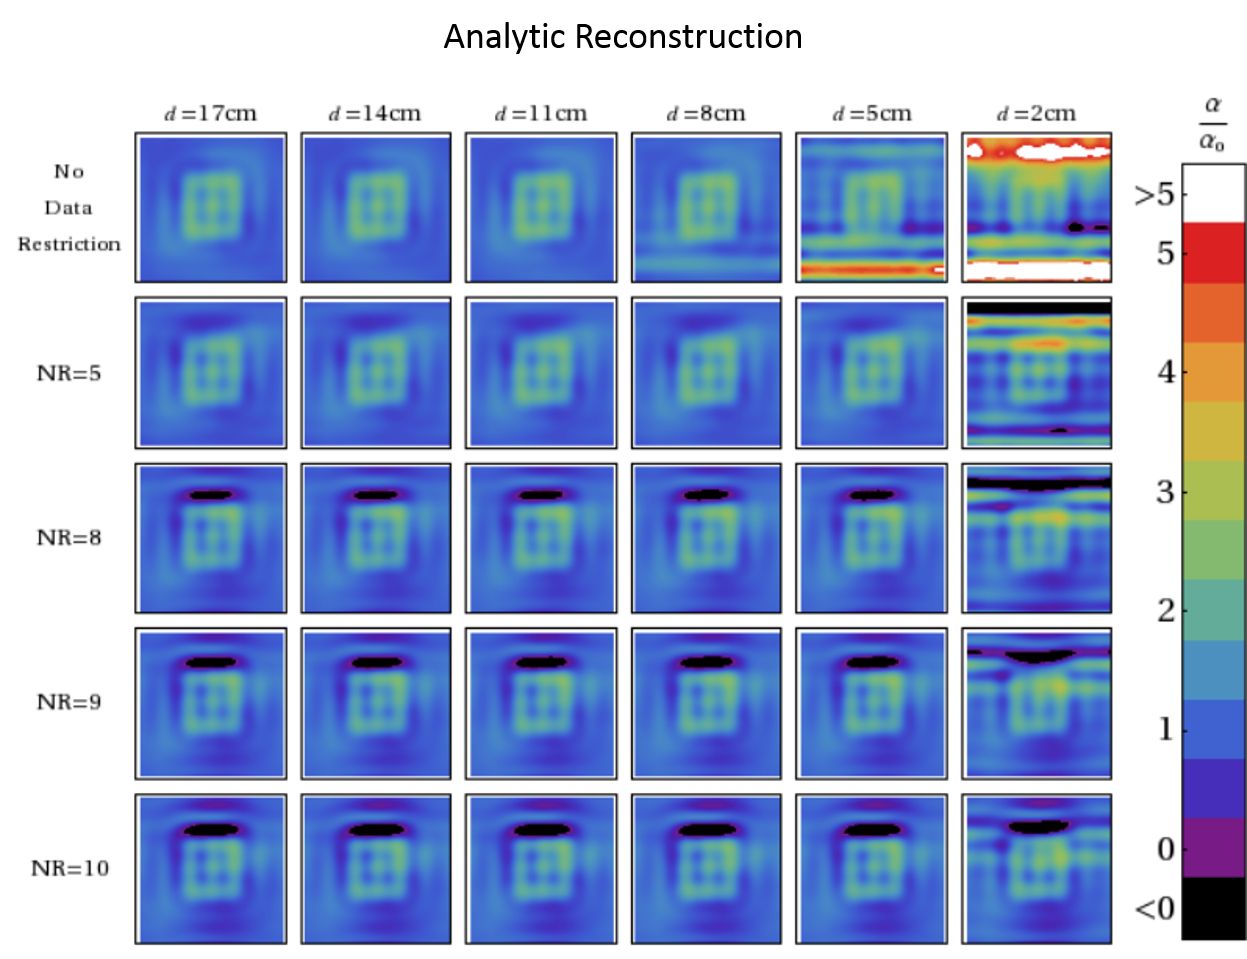
\includegraphics[width=0.9\textwidth]{./figures/3_Chestwall/fastcenter.png}
\caption[Images of the central slice obtained by analytical reconstruction method]{\label{fig:fastcenter}
Images of the central slice obtained by analytical reconstruction method. Different columns show data obtained with the chest wall phantoms at different distances $d$ from the bar target. Different rows of images correspond to different data restrictions $NR$, as indicated.}
\end{figure}

\begin{figure}[htbp]
\centering
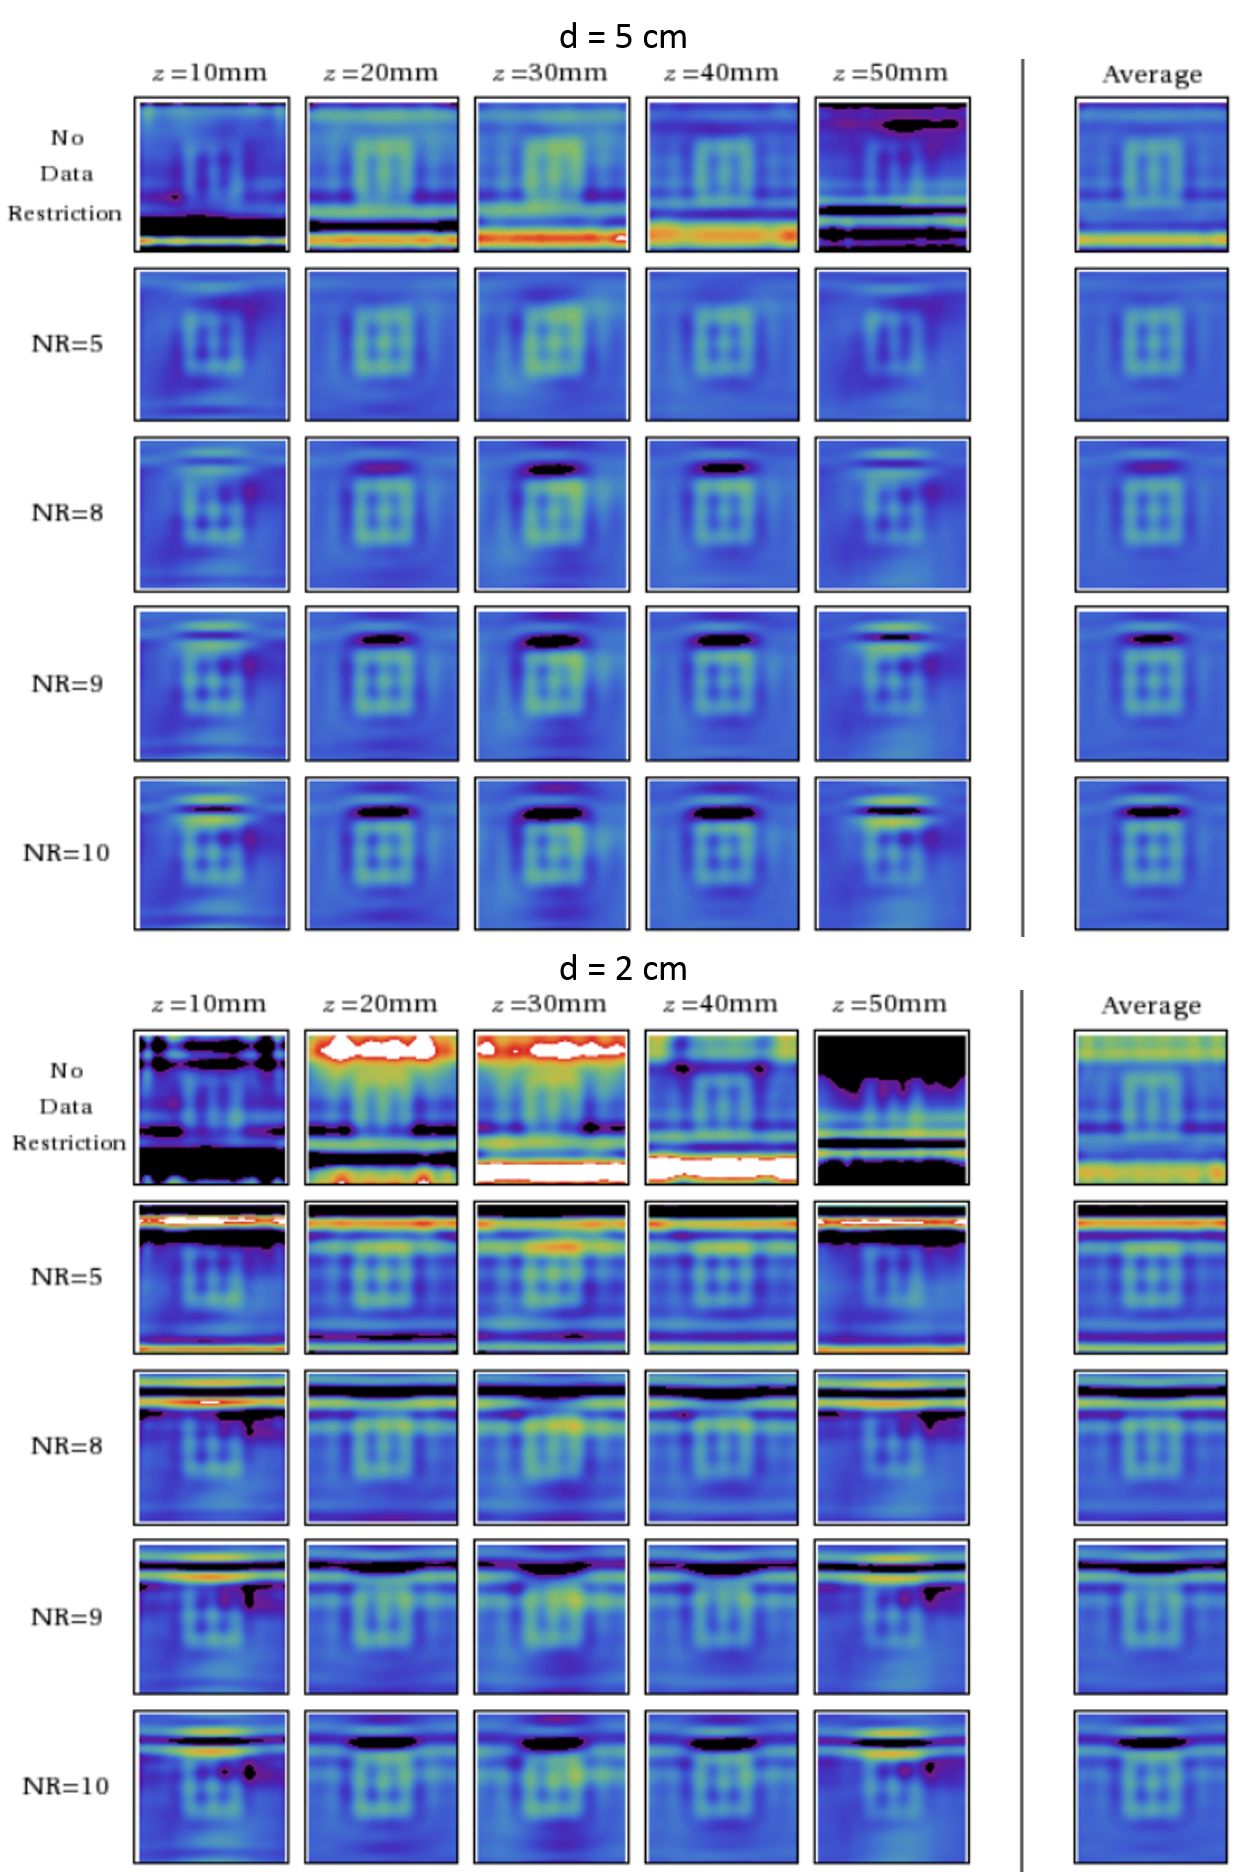
\includegraphics[width=0.9\textwidth]{./figures/3_Chestwall/anaslices.png}
\caption[Analytical reconstruction images at various depths]{\label{fig:slices_analytical}
Slices through the medium drawn at different depths (from plane of sources). The analytical inversion reconstruction method used for $d=5\,\rm{cm}$ and $d=2\,\rm{cm}$.}
\end{figure}
Interestingly, when the data restriction $NR = 8, 9, 10$ is used in conjunction with the analytical reconstruction, it yields an additional image artifact, which is unrelated to the chest wall phantom. To see that this is true, consider the images for $d=17\,{\rm cm}$, which are not affected at all by the chest wall phantom, yet exhibit the additional artifact just mentioned. This artifact is evident as a black area wherein the reconstructed absorption coefficient is negative; therefore, it is outside of the physically-allowable range. Thus, it is reasonable to conclude that reconstructing the target via the analytical reconstruction method is feasible, especially with the use of the appropriate data restriction, but additional image artifacts can arise where the absorption is underestimated. 

In fact, the appearance of this artifact can be understood. As mentioned above, the data restriction used with the analytical reconstruction amounts to assuming that the truncated data points are zero. In other words, if it is assumed (even in the presence of the target) that the truncated source-detector pairs would have measured the same intensity as in the homogeneous slab, then $I(\mbf{r}_d,\mbf{r}_s) = I_0(\mbf{r}_d,\mbf{r}_s)$ for the truncated source-detector pairs (see Section~\ref{sec:rytov}, Chapter 2). The reconstruction algorithm seeks a contrast function $\delta\alpha(\mbf{r})$, which is compatible with this assumption.  For a purely absorbing target, however, the actual intensity $I(\mbf{r}_d,\mbf{r}_s)$ is smaller than $I_0(\mbf{r}_d,\mbf{r}_s)$ when at least one of the points $\mbf{r}_d,\mbf{r}_s$ is located not too far from the target (in the lateral direction) due to increased optical absorption. Whenever such data points are discarded, an artifact with negative $\delta\alpha$ is produced by the reconstruction algorithm to compensate for the absorption in the target. It can be seen that this artifact is located between the target and the region of source-detector pairs, which have been discarded. Of course, this analysis applies to the case when the position and optical contrast of the target is known.  In general, it may be difficult to predict the position of this artifact or to distinguish it from a true occurrence of negative $\delta\alpha$. There may also be a spatial overlap of the artifact and a true inhomogeneity.

\subsection{Algebraic Reconstruction Results}
In the algebraic reconstructions in Fig.~\ref{fig:algcenter} with the unrestricted data set, the image quality is still poor when the chest wall is to close. However, when the data restriction is gradually introduced these artifacts disappear. In the case $NR=10$ and $d=2\,{\rm cm}$ (the image in the bottom right corner), the target is clearly visible, and the image quality is about the same as with the use of the unrestricted data set and $d=17\,{\rm cm}$. Thus, introduction of data restriction does not result in substantively additional image artifacts or image quality degradation when the algebraic method is used.
\begin{figure}[h]
\centering
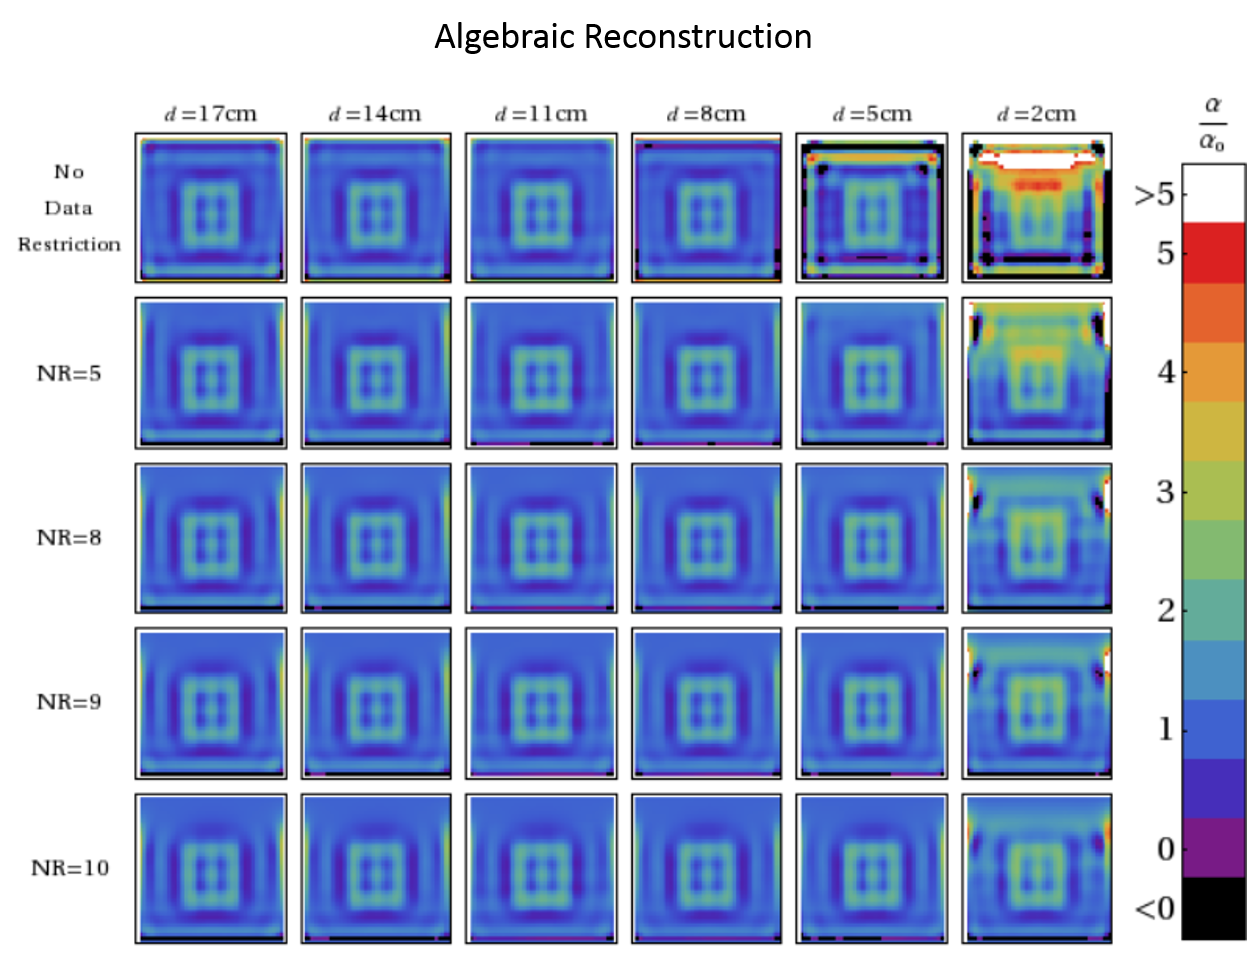
\includegraphics[width=0.9\textwidth]{./figures/3_Chestwall/algcenter.png}
\caption[Images of the central slice obtained by algebraic reconstruction method]{\label{fig:algcenter}
Images of the central slice obtained by algebraic reconstruction method. Different columns show data obtained with the chest wall phantoms at different distances $d$ from the bar target.  Different rows of images correspond to different data restrictions $NR$, as indicated.}
\end{figure}
\begin{figure}[p]
\centering
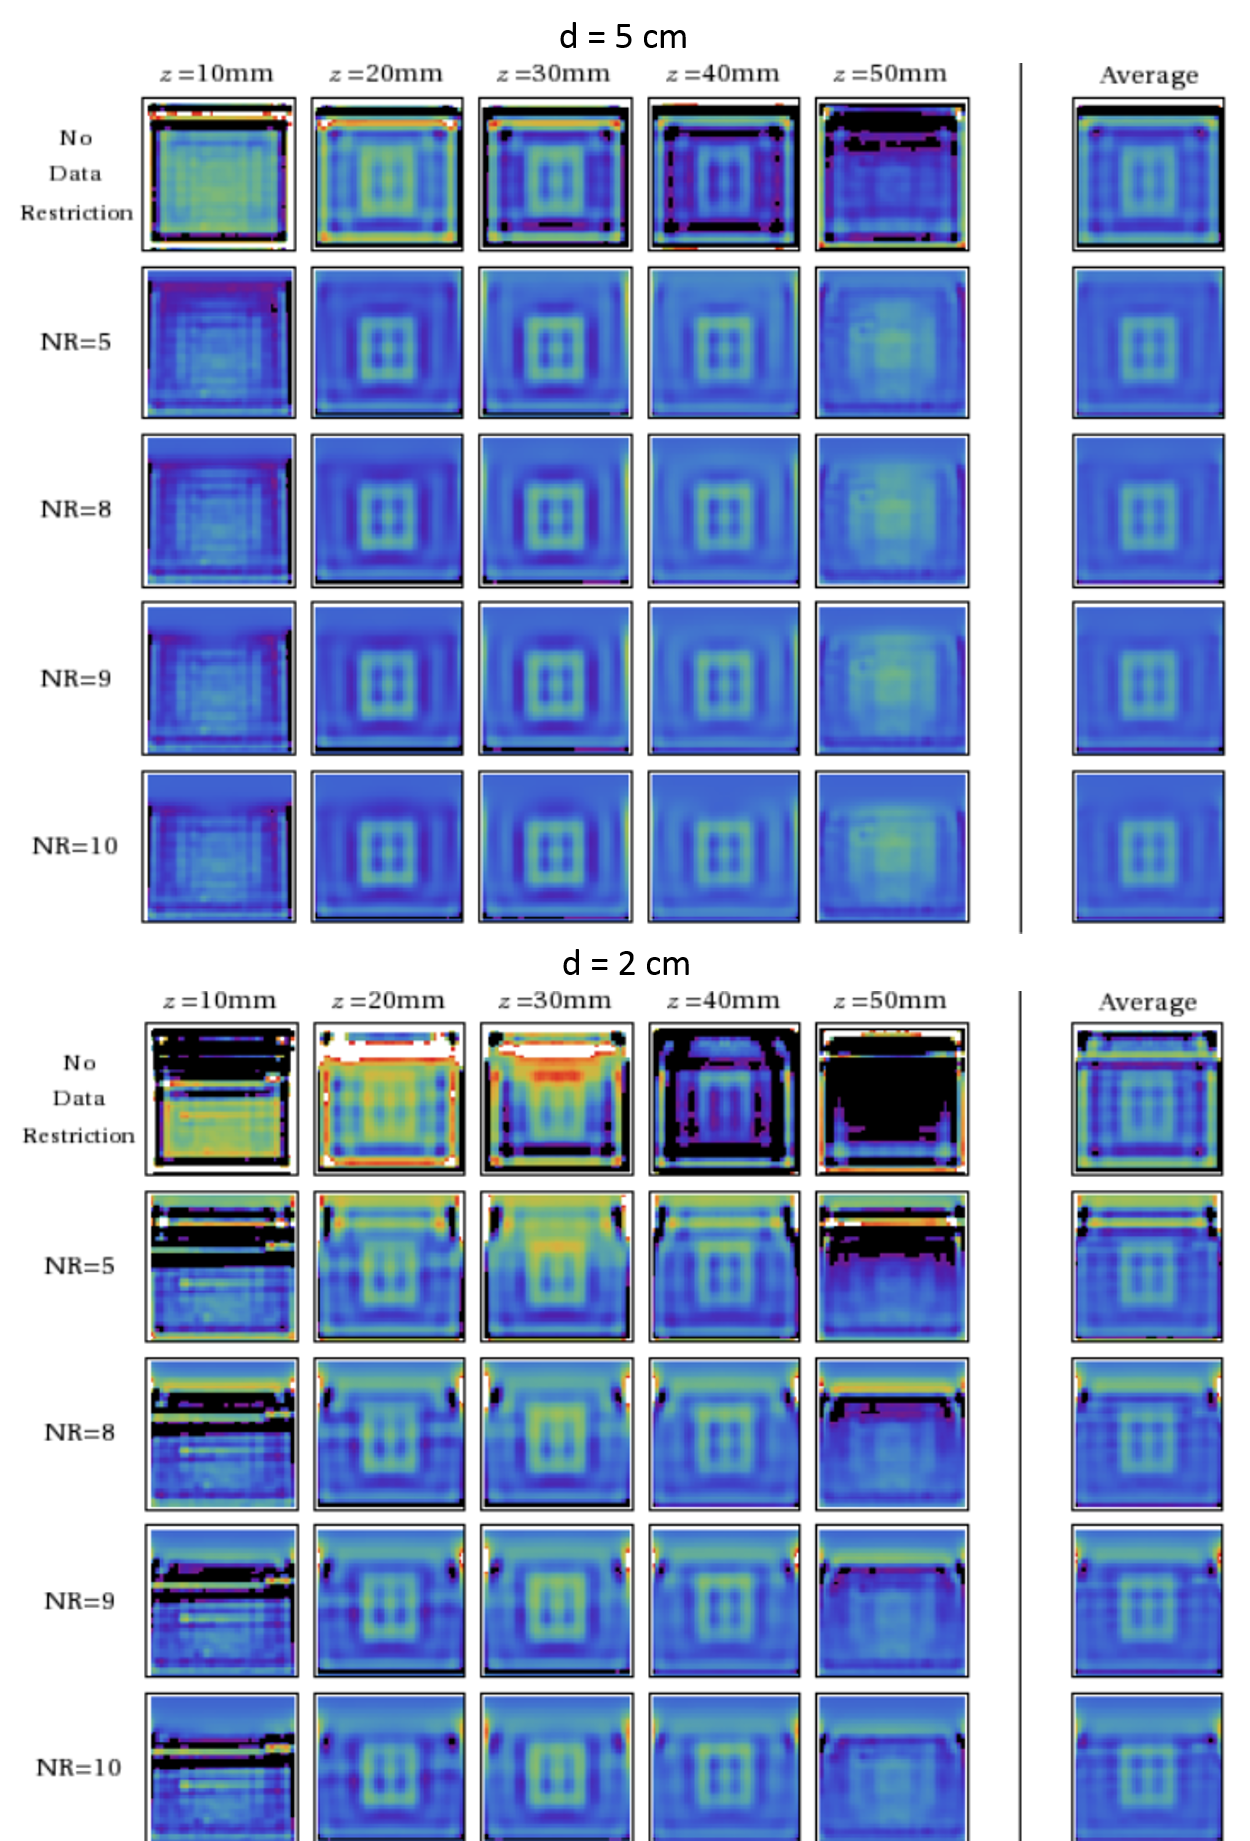
\includegraphics[width=0.9\textwidth]{./figures/3_Chestwall/algslices.png}
\caption[Algebraic reconstruction images at various depths]{Same as in Fig.~\ref{fig:slices_analytical}, but I this case the images are obtained by algebraic reconstruction}
\label{fig:slices_numerical}
\end{figure}

\subsection{Comparison of Reconstruction methods and Projection Images}
Figs.~\ref{fig:slices_analytical} and \ref{fig:slices_numerical} show slices drawn through the medium at different depths. Fig.~\ref{fig:slices_analytical} displays the results of the analytical image reconstruction for $d=5\,{\rm cm}$ and $d=2\,{\rm cm}$ and Fig.~\ref{fig:slices_numerical} displays analogous data obtained by the algebraic reconstruction. In addition, in the right-most column of images, a different kind of image is shown; these images are reconstructions derived by averaging the full 3D tomogram over the depth of the sample (that is, averaging over the different slices). Note that, in all cases $13$ slices in the tomogram are separated by the distance of $\approx 3.328{\rm mm}$, with the central slice located exactly in the mid-plane of the slab. The ``average'' reconstruction (in the right-most column of the images) was obtained by computing the arithmetic average of all $13$ slices.

These averaged (``projection'') images correspond to the usual radiological projections obtained with a parallel beam of X-rays. Interestingly, the qualitative conclusions that can be drawn from Figs.~\ref{fig:slices_analytical} and \ref{fig:slices_numerical} are largely the same as given above for the full tomograms. The analytical reconstruction produces reasonable image quality for the smallest chest wall-target separation $d=2\,{\rm cm}$ and $NR=10$, but at the cost of an additional image artifact. The algebraic reconstruction is free from this artifact, but it underestimates the image contrast relative to the analytic method (see below). The depth resolution is slightly better in algebraic reconstructions but, overall (i.e., in both methods), depth resolution is worse than lateral resolution. This effect is typical for DOT images.

Another interesting feature can be discerned from both types of image reconstructions. Generally, the projection images discussed above are more stable and exhibit reasonable quality even when the individual slices contain substantial artifacts. For example, consider the $d=2\,{\rm cm}$ algebraic reconstructions without data restriction (Fig.~\ref{fig:slices_numerical}). Even though all slices drawn through the medium are corrupted by the artifacts associated with proximity of the chest wall phantom, the projection image shows the target clearly. Moreover, the edge of the chest wall phantom is also clearly visible at the correct location. I was surprised, and indeed our group was surprised by this result. It can be useful in situations when the depth resolution is not of essence. However, it should be emphasized that obtaining the projections still requires knowledge of the three-dimensional distribution of the absorption coefficient; the projections cannot be computed or measured directly without such knowledge.

Finally, note that in both types of image reconstructions, an underestimation of the contrast for the target phantom is observed compared to the expected value. This underestimation can be attributed to the poor transverse (depth) resolution of the three-dimensional reconstruction which results in the ``spreading'' of the contrast in that direction. Indeed, consider the depth-integrated contrast, $H(x,y) = \int \left[\alpha(x,y,z) / \alpha_0 - 1 \right] {\rm d}z$, where $x$, $y$ are the coordinates in the plane of the slab and $z$ is the transverse (depth) coordinate. Inside the target, $\alpha(x,y,z) / \alpha_0 \simeq 4$ and the target thickness in the transverse direction is $\Delta z=0.6\,\ {\rm cm}$. Therefore, the actual value of $H$ for a line passing through the target and perpendicularly to the slab surface is $H\simeq 1.8\,{\rm cm}$. In the reconstructed images, the transverse thickness of the target is overestimated and is equal, approximately, to $2\,{\rm cm}$ while the quantity $\alpha(x,y,z)/\alpha_0$ is underestimated and is equal, approximately, to 2. By using the reconstructed values to estimate the integrated contrast, one obtains $H\simeq 2\,{\rm cm}$, which is reasonably close to the actual value. Again, this effect (and analysis scheme) can be useful in practice.

\section{Summary}
\label{sec:3_summary}
The aim of my experiment was to assess the effects of the chest wall on DOT and ultimately to explore methods to mitigate the effect of the chest wall on DOT reconstructions. Both the analytical and the algebraic data-intensive linearized image reconstruction methods produce reasonable results, provided the data points are appropriately restricted to exclude measurements that are strongly influenced by the chest wall. Under these conditions, an absorbing target with sub-ccentimeter features can be clearly reconstructed in the middle of a $6$ cm slab, even when the chest wall is only $2$ cm from the target. This situation corresponds to breast tumors very near the chest wall. Specifically, good images of the target were obtained even in the presence of a large chest wall phantom that introduces significant nonlinearities into the inverse problem,  i.e., due to its larger absorption coefficient compared to the background as well as its large size. 

A data restriction condition was discovered such that the presence of the chest wall phantom imposes minimal artifacts or distortions in the image. The image quality of the projections was good and it would be of interest to explore the utility of these reconstructions for improved 2D imaging or improved quantification or in combination with other 2D modalities. The performance of both algebraic and analytic image reconstruction methods were then compared under this condition and, while neither method is perfect, it appears that a role for both methods in DOT exists, the choice depending upon the particular clinical application. For example, the analytical method provides faster reconstruction while suffering from minor artifacts and flexibility. While the algebraic reconstruction method provides slightly better image quality, it will require a library of weight matrices for faster inversion that would have to be stored ahead of time before measurements (see Section~\ref{sec:Algebraic}. We hope to build on these techniques in the future, especially by implementing non-linear approaches or by modification of the Green's function used to account for the chest wall region and its optical properties.